\documentclass[tikz, border=2pt]{standalone}
\usepackage{amsmath, amssymb}
\usepackage{pgfplots}
\pgfplotsset{compat=1.18}
\usetikzlibrary{arrows.meta}

\definecolor{oxfordblue}{RGB}{0,33,71}
\definecolor{posteriorblue}{RGB}{60,120,200}
\definecolor{priorgray}{RGB}{160,160,160}

\begin{document}
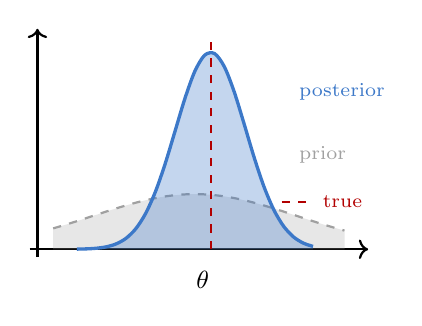
\begin{tikzpicture}

	\draw[->, thick] (-0.1,0) -- (4.2,0);
	\draw[->, thick] (0,-0.1) -- (0,2.8);
	\node[font=\small, anchor=north] at (2.1,-0.15) {$\theta$};

	% Prior (wide, flat)
	\fill[priorgray, opacity=0.25]
		plot[smooth, domain=0.2:3.9] (\x, {0.7*exp(-0.3*(\x-2.0)^2)}) -- (3.9,0) -- (0.2,0) -- cycle;
	\draw[thick, priorgray, dashed]
		plot[smooth, domain=0.2:3.9] (\x, {0.7*exp(-0.3*(\x-2.0)^2)});

	% Posterior (narrow, tall)
	\fill[posteriorblue, opacity=0.3]
		plot[smooth, domain=0.5:3.5] (\x, {2.5*exp(-2.5*(\x-2.2)^2)}) -- (3.5,0) -- (0.5,0) -- cycle;
	\draw[very thick, posteriorblue]
		plot[smooth, domain=0.5:3.5] (\x, {2.5*exp(-2.5*(\x-2.2)^2)});

	% True value
	\draw[thick, red!70!black, dashed] (2.2,0) -- (2.2,2.7);

	% Legend
	\node[font=\scriptsize, priorgray, anchor=west] at (3.2,1.2) {prior};
	\node[font=\scriptsize, posteriorblue, anchor=west] at (3.2,2.0) {posterior};
	\draw[thick, red!70!black, dashed] (3.1,0.6) -- (3.5,0.6);
	\node[font=\scriptsize, red!70!black, anchor=west] at (3.5,0.6) {true};

\end{tikzpicture}
\end{document}
